\documentclass[tikz,border=2mm]{standalone}

\usepackage{bm}
\usepackage{xcolor}
\usetikzlibrary{arrows,positioning}
\usetikzlibrary{arrows.meta}

\newcommand{\VE}{\ensuremath{\textrm{VE}}}

\definecolor{colorS}{HTML}{56B4E9}
\definecolor{colorRu}{HTML}{009E73}
\definecolor{colorV}{HTML}{F0E442}
\definecolor{colorRv}{HTML}{D55E00}
\definecolor{colorIu}{HTML}{0072B2}
\definecolor{colorIv}{HTML}{E69F00}

\begin{document}

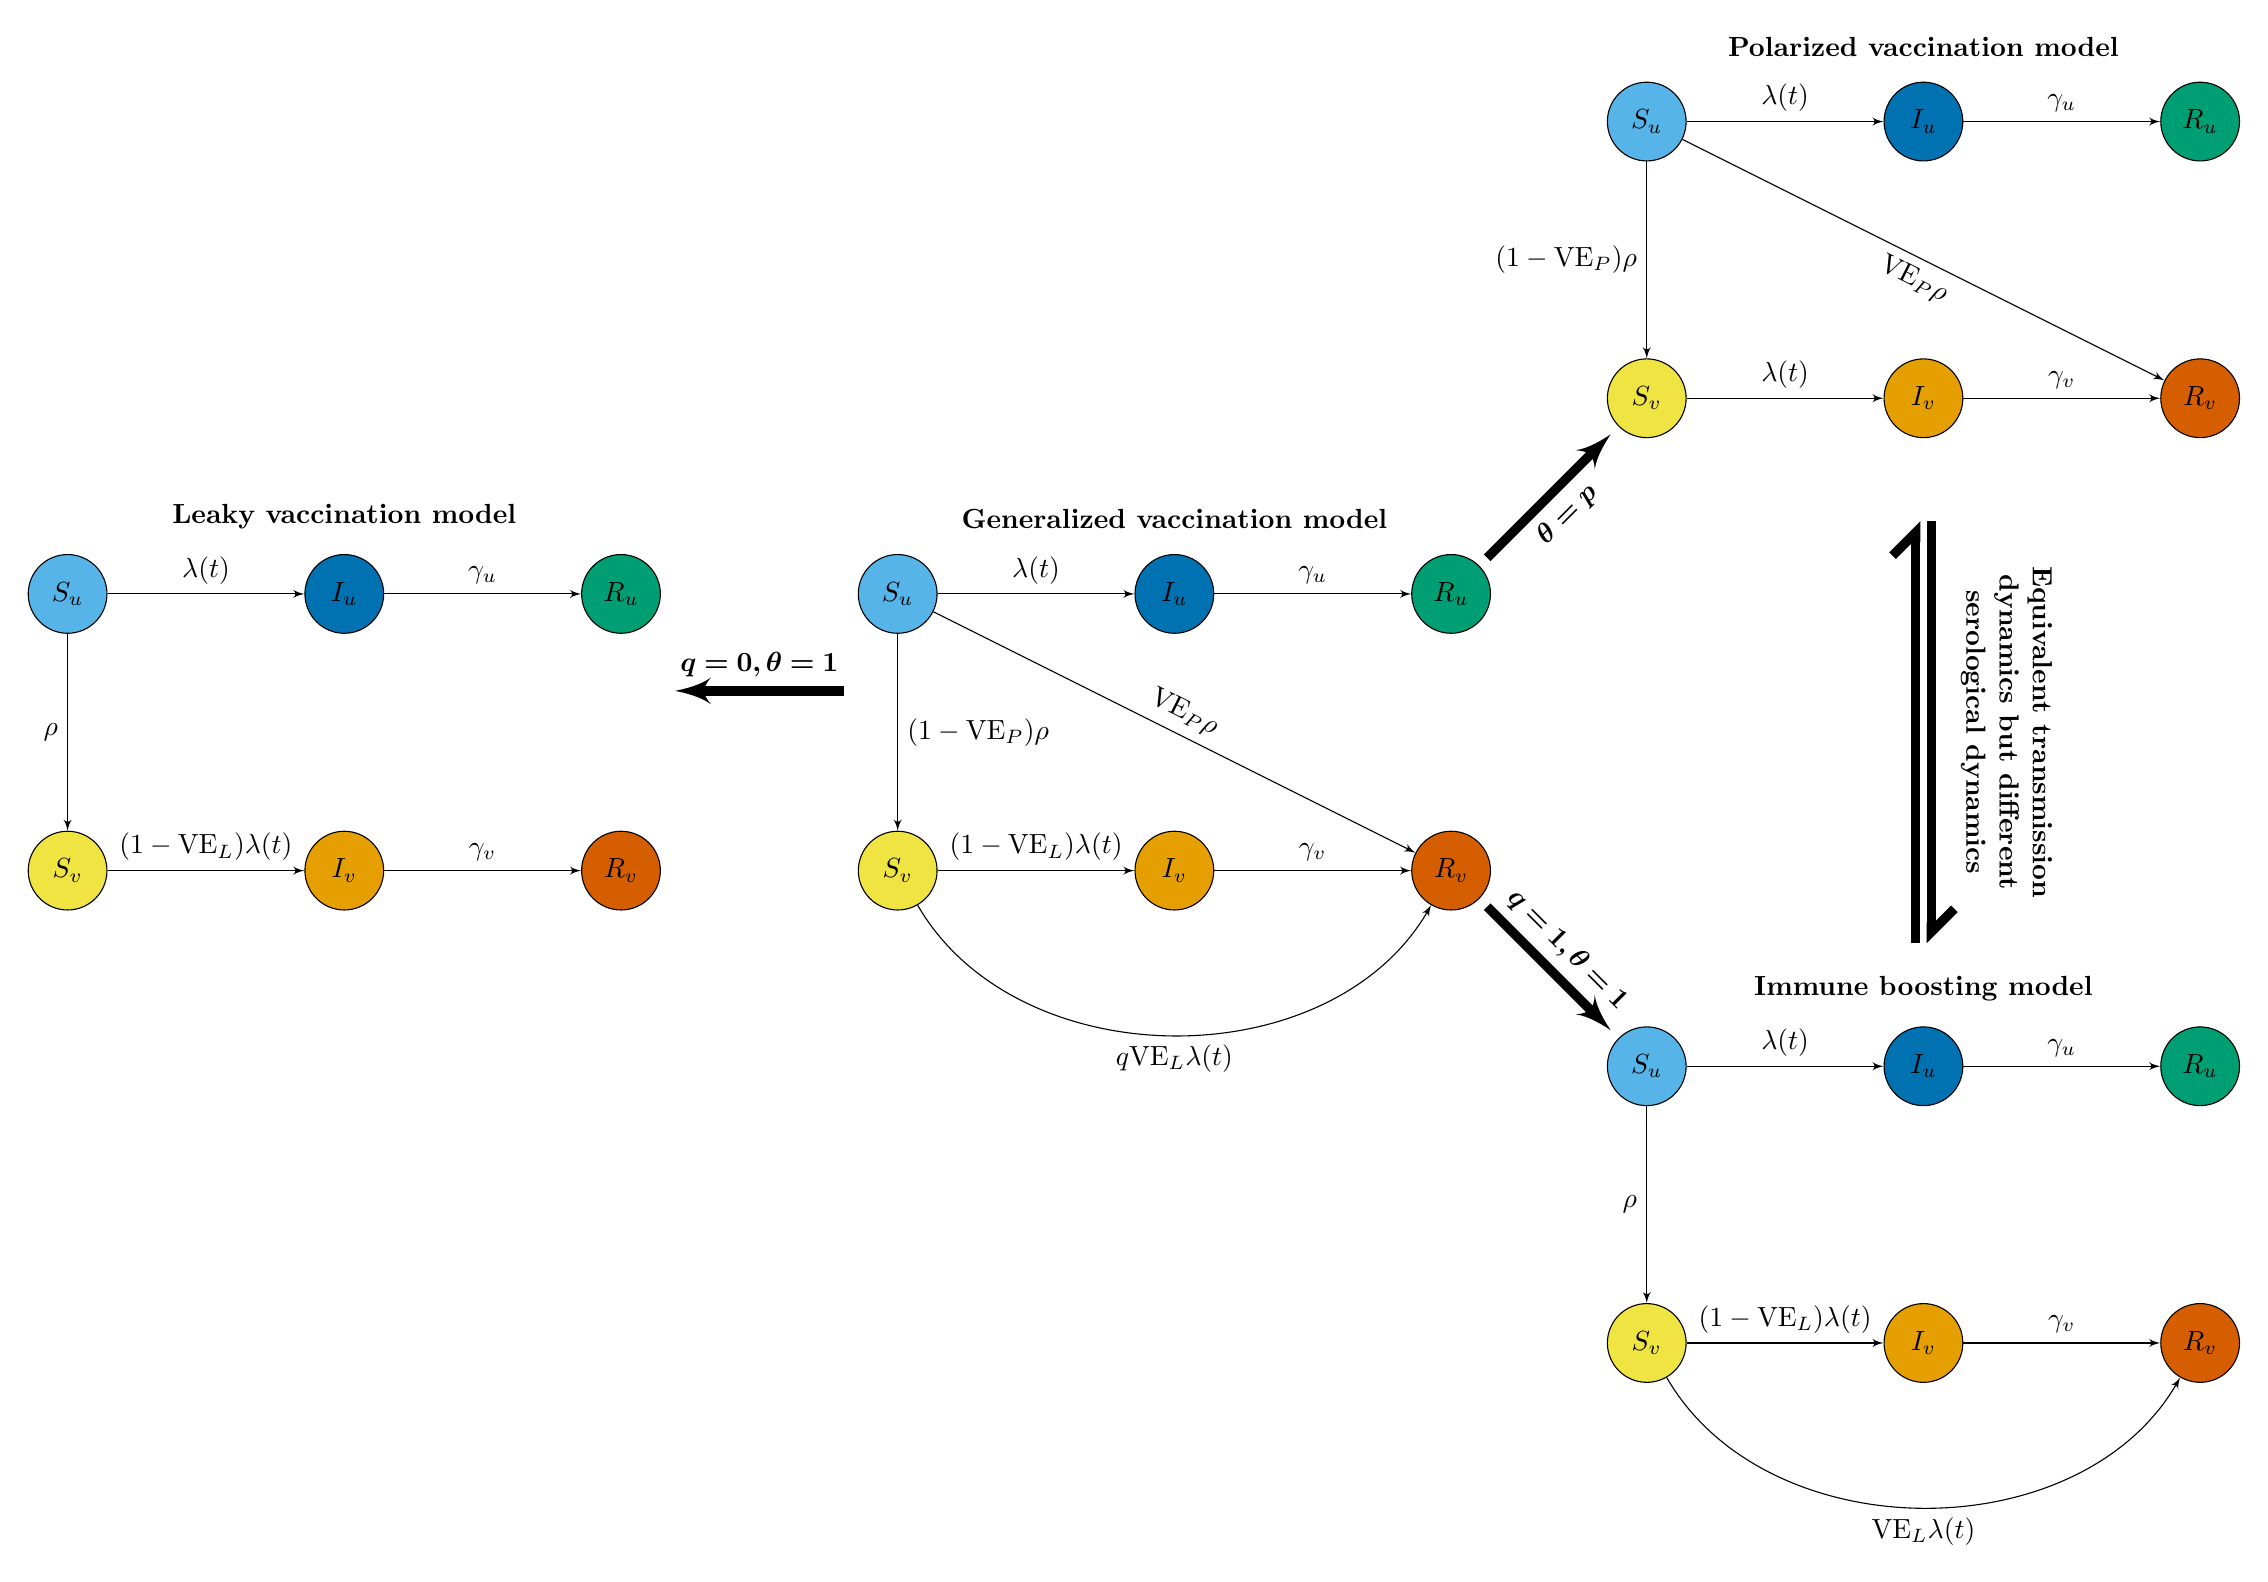
\begin{tikzpicture}[node distance=2.5cm,auto,>=latex',every node/.append style={align=center},int/.style={draw, minimum size=1cm, circle},inverter/.style={rectangle,draw,inner sep=2pt,minimum size=6mm},]
    \node [int, fill=colorS, fill opacity=1, text opacity=1] (S)             {$S_u$};
    \node [int, right=of S, fill=colorIu] (Is)             {$I_u$};
    \node [int, right=of Is, fill=colorRu, fill opacity=1, text opacity=1] (Rs)             {$R_u$};
    \path[->] (S) edge node [above] {$\lambda(t)$}  (Is);
    \path[->] (Is) edge node [above] {$\gamma_u$} (Rs);
    \node [int, below=of S, fill=colorV, fill opacity=1, text opacity=1] (V)             {$S_v$};
    \node [int, right=of V, fill=colorIv] (Iv)             {$I_v$};
    \node [int, right=of Iv, fill=colorRv, fill opacity=1, text opacity=1] (Rv)             {$R_v$};
    \path[->] (S) edge node [left] {$\rho$} (V);
    \path[->] (V) edge node [above] {$(1-\VE_L) \lambda(t)$}(Iv);
    \path[->] (Iv) edge node [above] {$\gamma_v$} (Rv);
    \node [int, right=2.5cm of Rs, fill=colorS, fill opacity=1] (S2)             {$S_u$};
    \node [int, right=of S2, fill=colorIu] (Is2)             {$I_u$};
    \node [int, right=of Is2, fill=colorRu, fill opacity=1, text opacity=1] (Rs2)             {$R_u$};
    \path[->] (S2) edge node [above] {$\lambda(t)$} (Is2);
    \path[->] (Is2) edge node [above] {$\gamma_u$} (Rs2);
    \node [int, below=of S2, fill=colorV, fill opacity=1, text opacity=1] (V2)             {$S_v$};
    \node [int, right=of V2, fill=colorIv] (Iv2)             {$I_v$};
    \node [int, right=of Iv2, fill=colorRv, fill opacity=1, text opacity=1] (Rv2)             {$R_v$};
    \path[->] (S2) edge node [right] {$(1-\VE_P) \rho$} (V2);
    \path[->] (S2) edge node [sloped, above] {$\VE_P \rho$} (Rv2);
    \path[->] (V2) edge node [above] {$(1-\VE_L) \lambda(t)$} (Iv2);
    \path[->] (Iv2) edge node [above] {$\gamma_v$} (Rv2);
    \path[->] (V2) edge [out=-60, in=-120] node [below] {$q \VE_L \lambda(t)$} (Rv2);
    \node [int, below right=2.5cm of Rv2, fill=colorS, fill opacity=1] (S3)             {$S_u$};
    \node [int, right=of S3, fill=colorIu] (Is3)             {$I_u$};
    \node [int, right=of Is3, fill=colorRu, fill opacity=1, text opacity=1] (Rs3)             {$R_u$};
    \path[->] (S3) edge node [above] {$\lambda(t)$} (Is3);
    \path[->] (Is3) edge node [above] {$\gamma_u$} (Rs3);
    \node [int, below=of S3, fill=colorV, fill opacity=1, text opacity=1] (V3)             {$S_v$};
    \node [int, right=of V3, fill=colorIv] (Iv3)             {$I_v$};
    \node [int, right=of Iv3, fill=colorRv, fill opacity=1, text opacity=1] (Rv3)             {$R_v$};
    \path[->] (S3) edge node [left] {$\rho$} (V3);
    \path[->] (V3) edge node [above] {$(1-\VE_L) \lambda(t)$} (Iv3);
    \path[->] (Iv3) edge node [above] {$\gamma_v$} (Rv3);
    \path[->] (V3) edge [out=-60, in=-120] node [below] {$\VE_L \lambda(t)$} (Rv3);
    \node [int, above right=2.5cm of Rs2, fill=colorV, fill opacity=1, text opacity=1] (V4)             {$S_v$};
    \node [int, above=of V4, fill=colorS, fill opacity=1, text opacity=1] (S4)             {$S_u$};
    \node [int, right=of S4, fill=colorIu] (Is4)             {$I_u$};
    \node [int, right=of Is4, fill=colorRu, fill opacity=1, text opacity=1] (Rs4)             {$R_u$};
    \path[->] (S4) edge node [above] {$\lambda(t)$} (Is4);
    \path[->] (Is4) edge node [above] {$\gamma_u$} (Rs4);
    \node [int, right=of V4, fill=colorIv] (Iv4)             {$I_v$};
    \node [int, right=of Iv4, fill=colorRv, fill opacity=1, text opacity=1] (Rv4)             {$R_v$};
    \path[->] (S4) edge node [left] {$(1-\VE_P) \rho$} (V4);
    \path[->] (S4) edge node [sloped, below] {$\VE_P \rho$} (Rv4);
    \path[->] (V4) edge node [above] {$\lambda(t)$} (Iv4);
    \path[->] (Iv4) edge node [above] {$\gamma_v$} (Rv4);
    \node [below=0.6cm of S2, white] (tmp1) {};
    \node [below=0.6cm of Rs, white] (tmp2) {};
    \path[->, line width=1.2mm, shorten >= 16pt, shorten <= 16pt] (tmp1) edge node [above] {$\bm{q=0, \theta=1}$} (tmp2);
    \path[->, line width=1.2mm, shorten >= 4pt, shorten <= 4pt] (Rv2) edge node [sloped, above] {$\bm{q=1, \theta=1}$} (S3);
    \path[->, line width=1.2mm, shorten >= 4pt, shorten <= 4pt] (Rs2) edge node [sloped, below] {$\bm{\theta=p}$} (V4);
    \path[-{Straight Barb[left]}, line width=1.2mm, shorten >= 30pt, shorten <= 30pt] ([xshift=-1mm]Is3.north) edge node [sloped, above] {} ([xshift=-1mm]Iv4.south);
    \path[-{Straight Barb[left]}, line width=1.2mm, shorten >= 30pt, shorten <= 30pt] ([xshift=1mm]Iv4.south) edge node [sloped, above=0.2cm] {\textbf{Equivalent transmission}\\\textbf{dynamics but different}\\\textbf{serological dynamics}} ([xshift=1mm]Is3.north);
    \node[above=0.2cm of Is] {\textbf{Leaky vaccination model}};
    \node[above=0.2cm of Is2] {\textbf{Generalized vaccination model}};
    \node[above=0.2cm of Is3] {\textbf{Immune boosting model}};
    \node[above=0.2cm of Is4] {\textbf{Polarized vaccination model}};
\end{tikzpicture}
\end{document}